\section{Identificación de vocales}
	\subsection{Análisis de DFT de las vocales}
	Calculando la \texttt{FFT} de las vocales, se procede a graficar la magnitud en \textit{dB}, para el intervalo $\left[ 0, 4000 \right]$~Hz. Se considera dos casos, uno donde la \texttt{FFT} se calcula con todos los valores de la señal y otro donde se calcula para el intervalo de muestras donde se encuentra la información de la vocal: 
	\begin{figure}[H]
		\center
		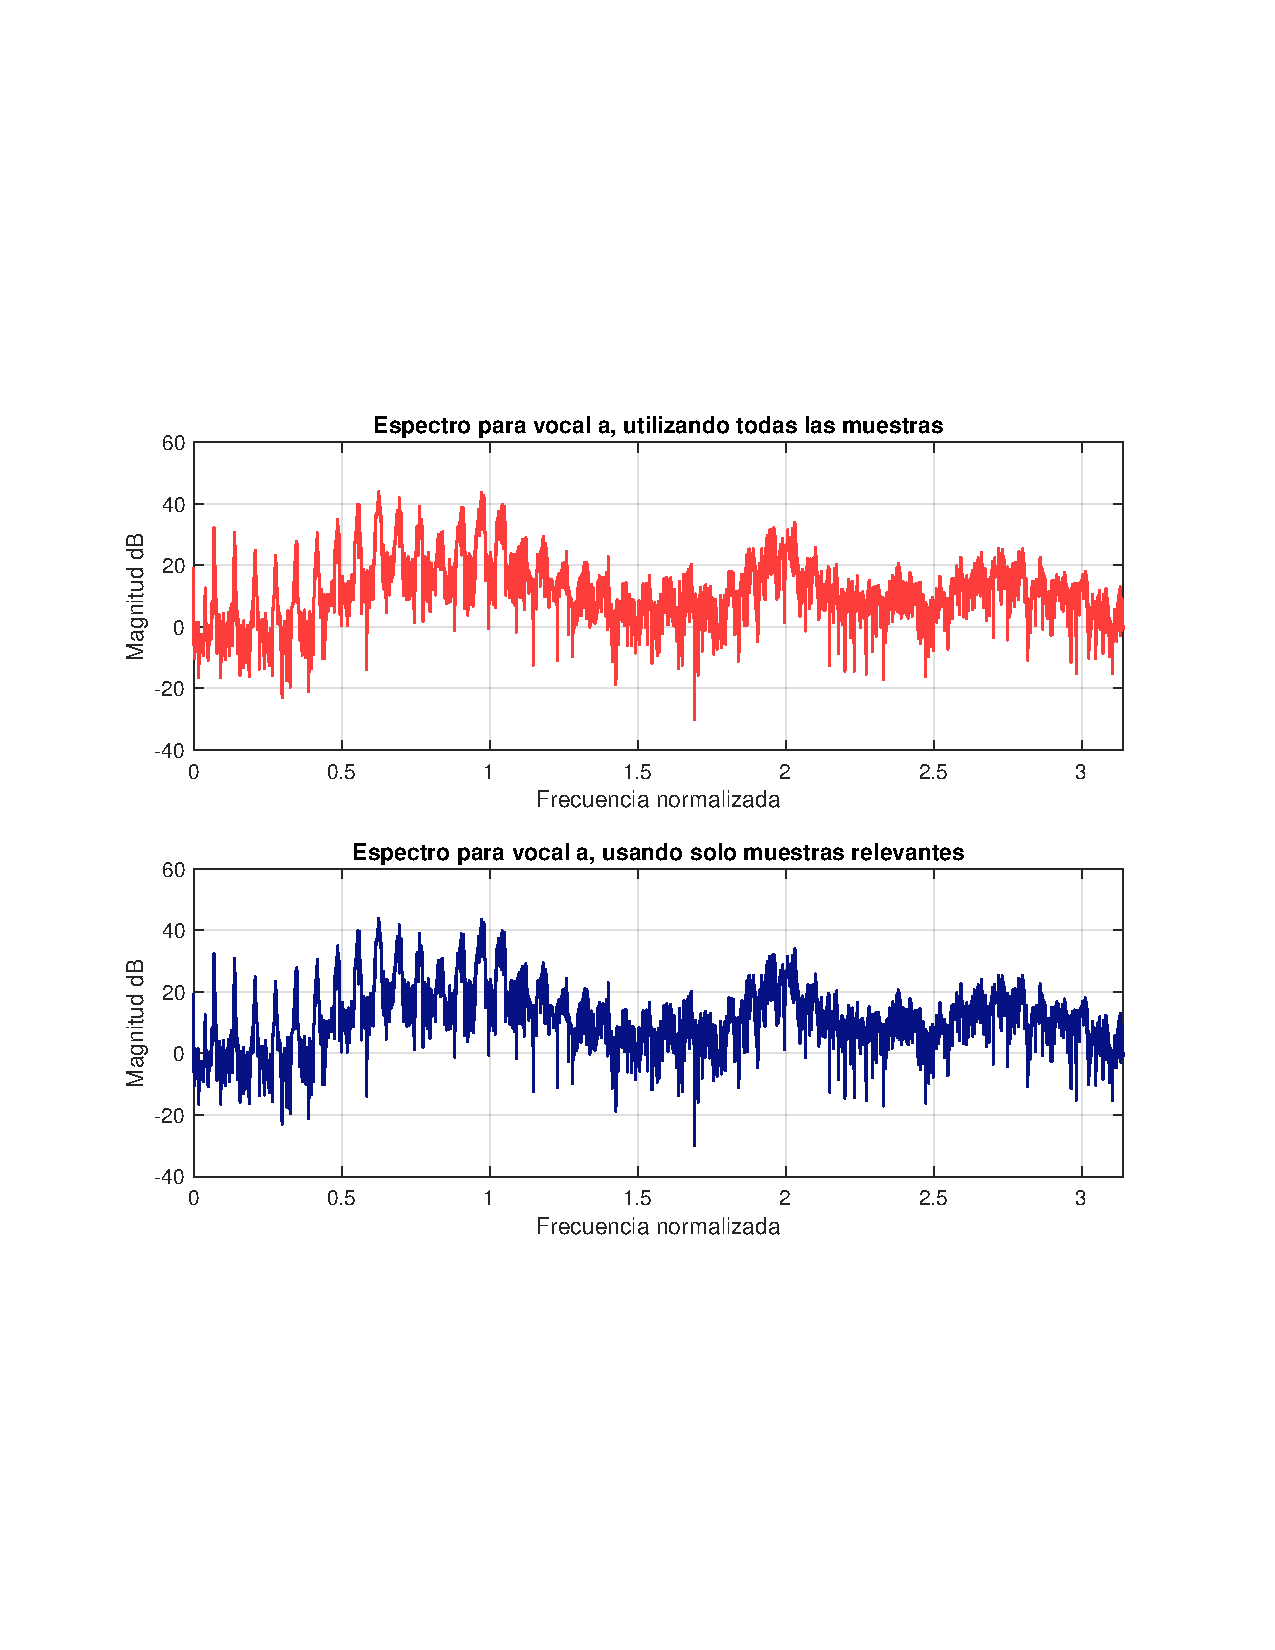
\includegraphics[width=0.6\textwidth,clip, trim = {1.9cm 6.8cm 2.3cm 7cm}]{../plots/a_fft.pdf}
		\caption{FFT para vocal a}
		\label{fig:a_fft}
	\end{figure}
	
	\begin{figure}[H]
		\center
		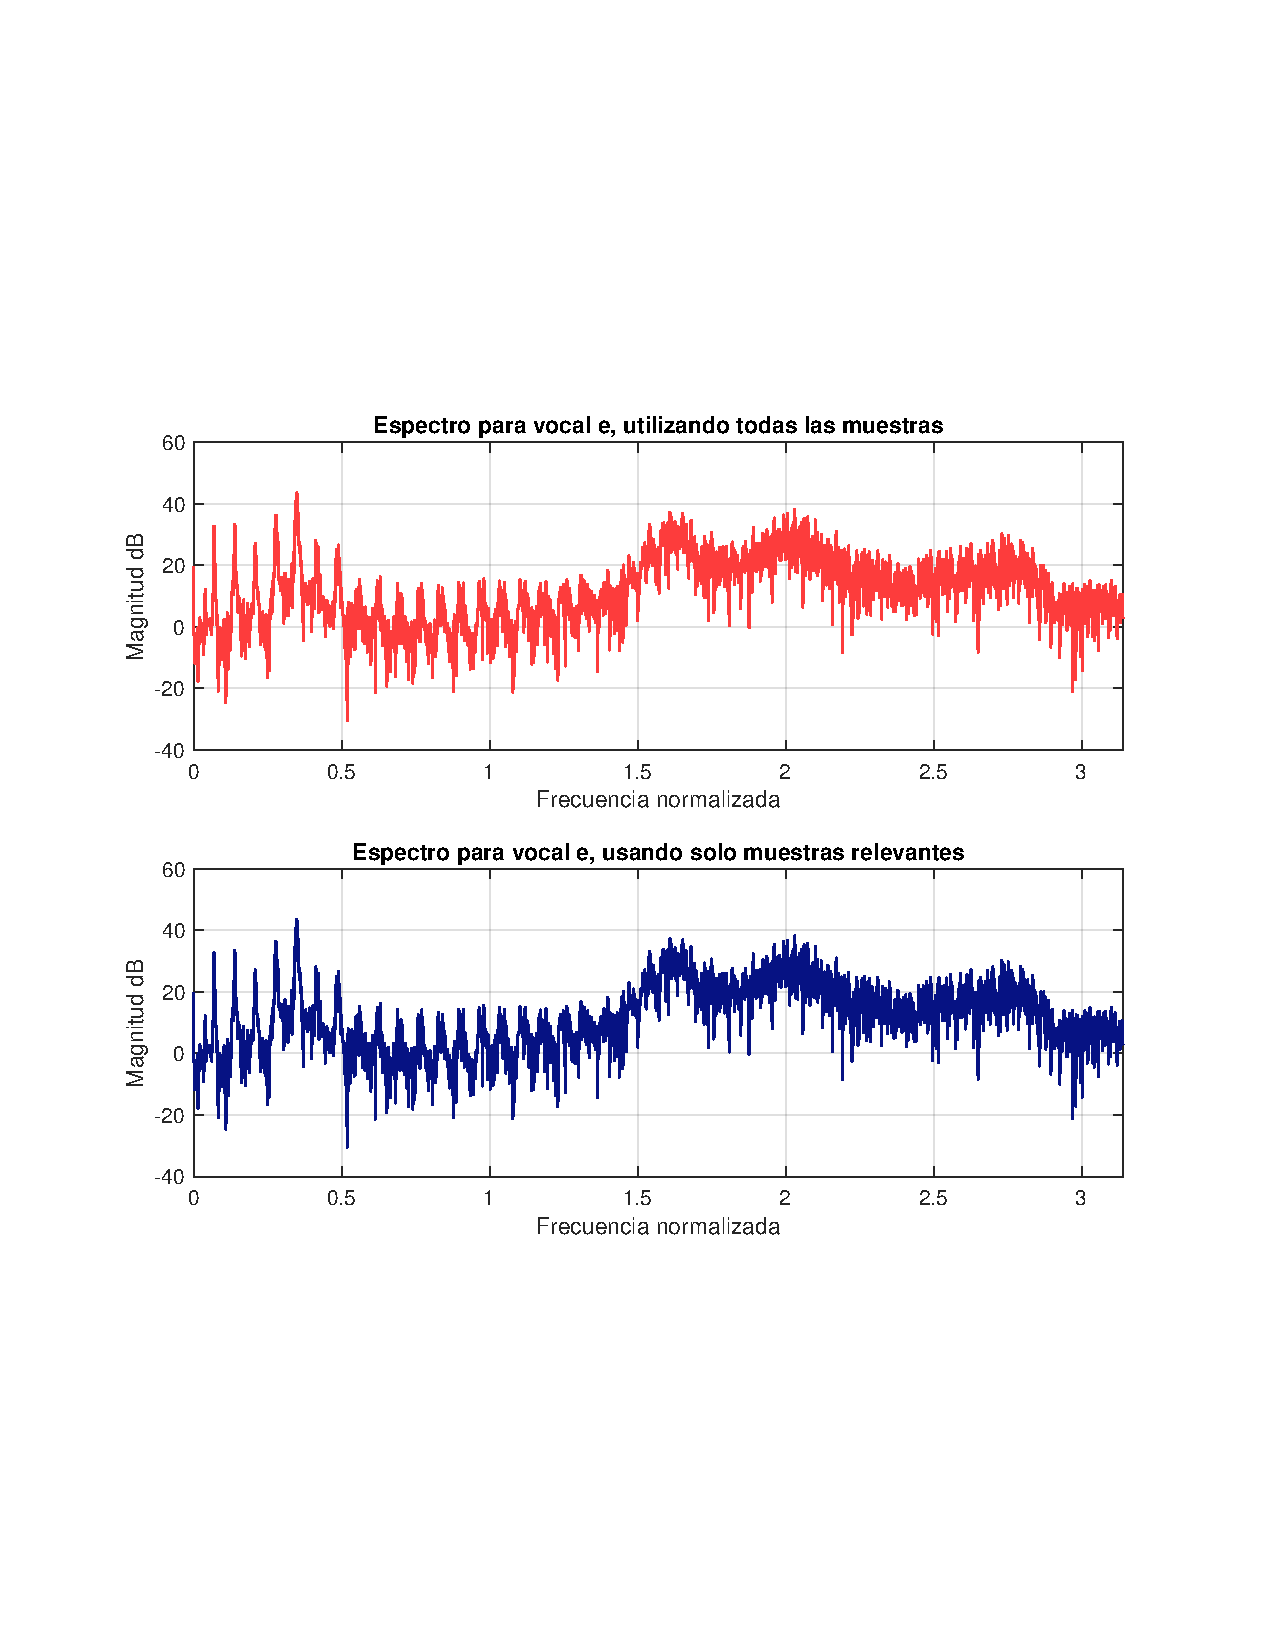
\includegraphics[width=0.6\textwidth,clip, trim = {1.9cm 6.8cm 2.3cm 7cm}]{../plots/e_fft.pdf}
		\caption{FFT para vocal e}
		\label{fig:e_fft}
	\end{figure}
	
	
	\begin{figure}[H]
		\center
		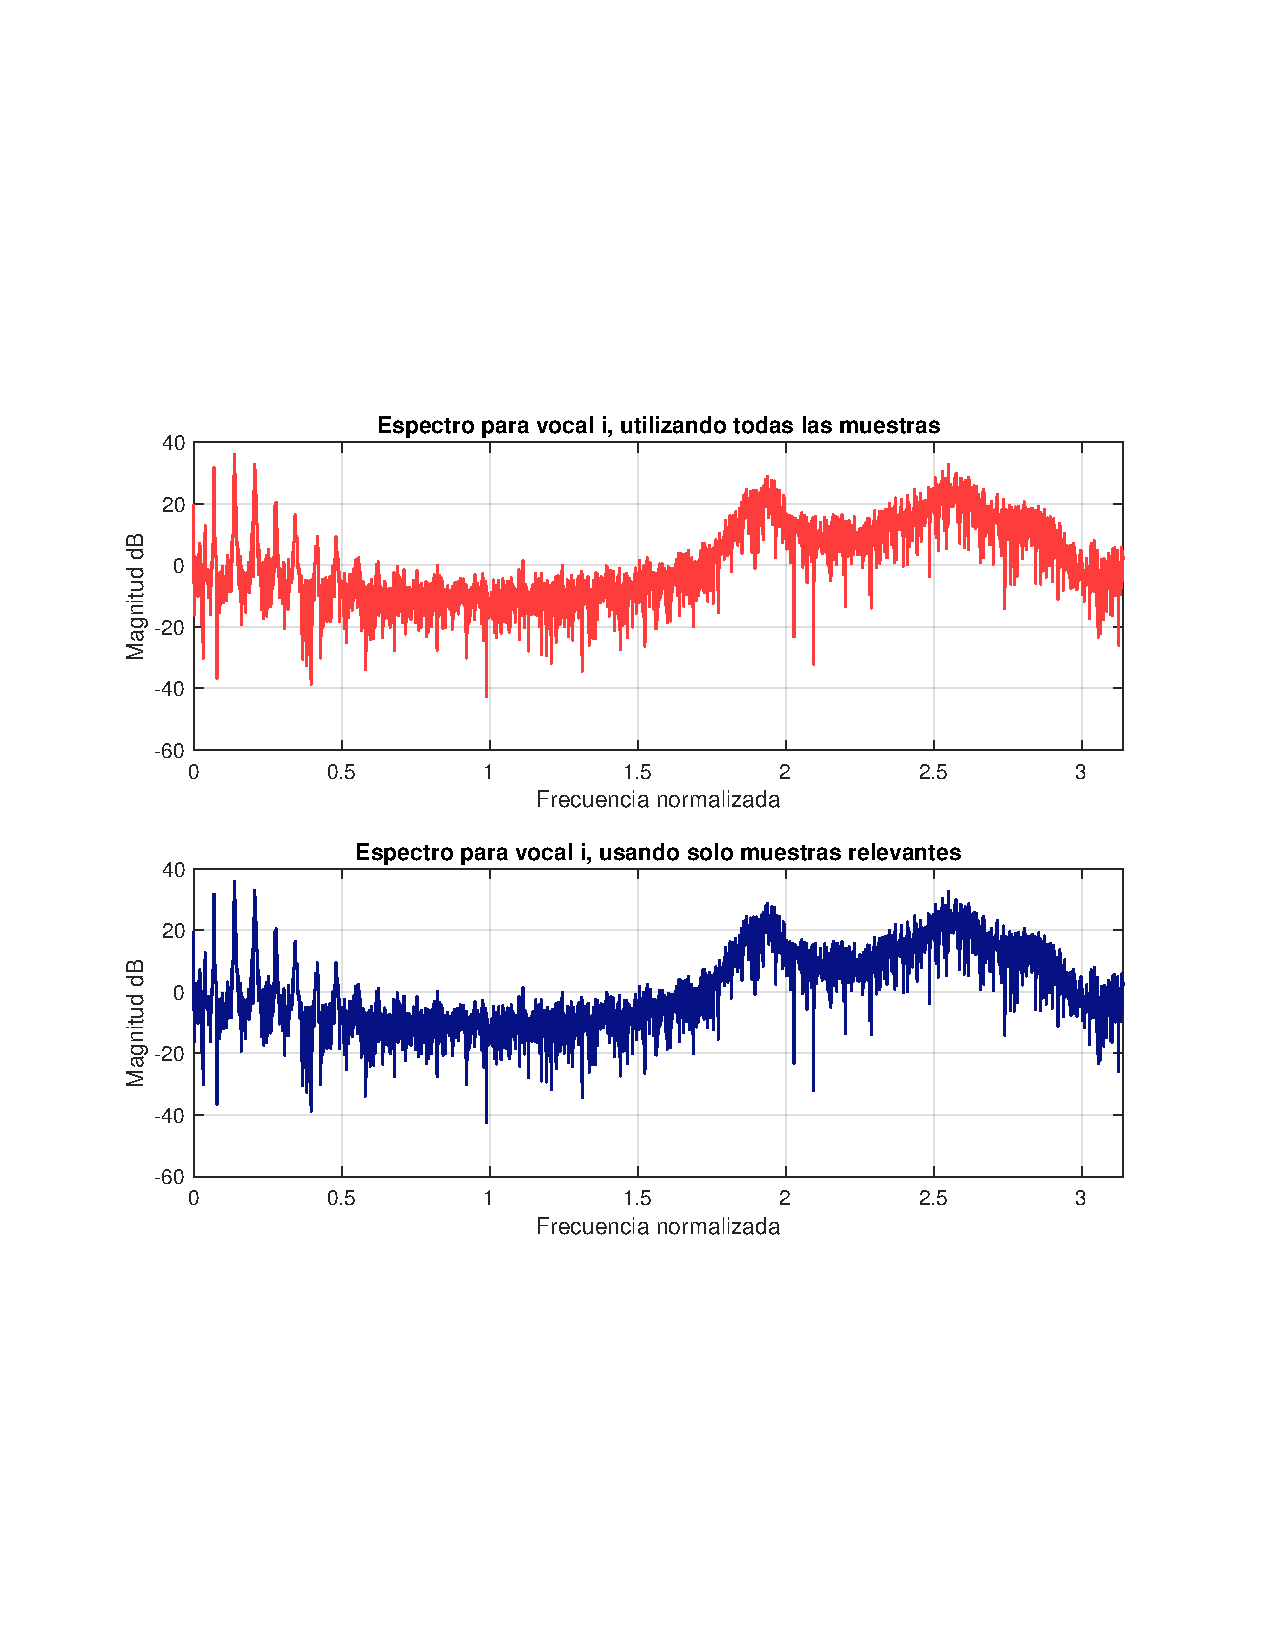
\includegraphics[width=0.6\textwidth,clip, trim = {1.9cm 6.8cm 2.3cm 7cm}]{../plots/i_fft.pdf}
		\caption{FFT para vocal i}
		\label{fig:i_fft}
	\end{figure}
	
	\begin{figure}[H]
		\center
		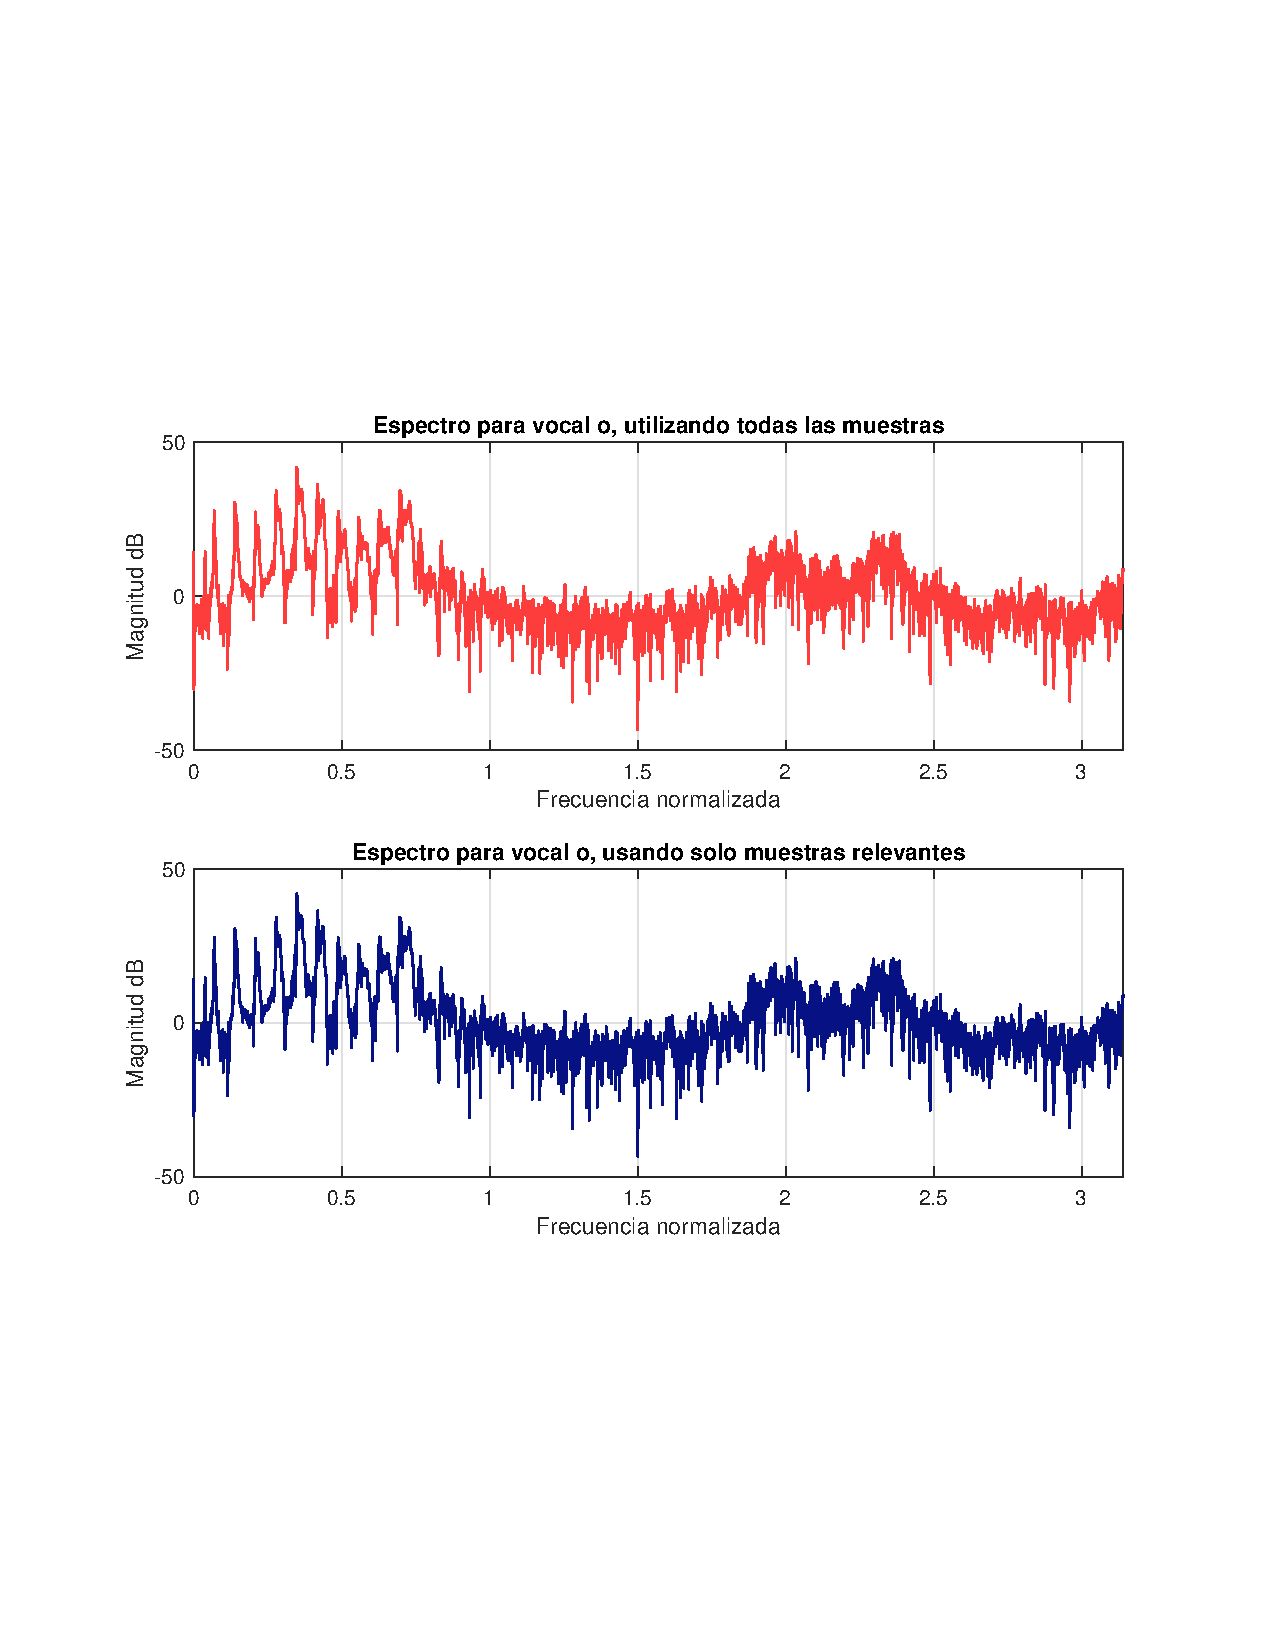
\includegraphics[width=0.6\textwidth,clip, trim = {1.9cm 6.8cm 2.3cm 7cm}]{../plots/o_fft.pdf}
		\caption{FFT para vocal o}
		\label{fig:o_fft}
	\end{figure}
	
	\begin{figure}[H]
		\center
		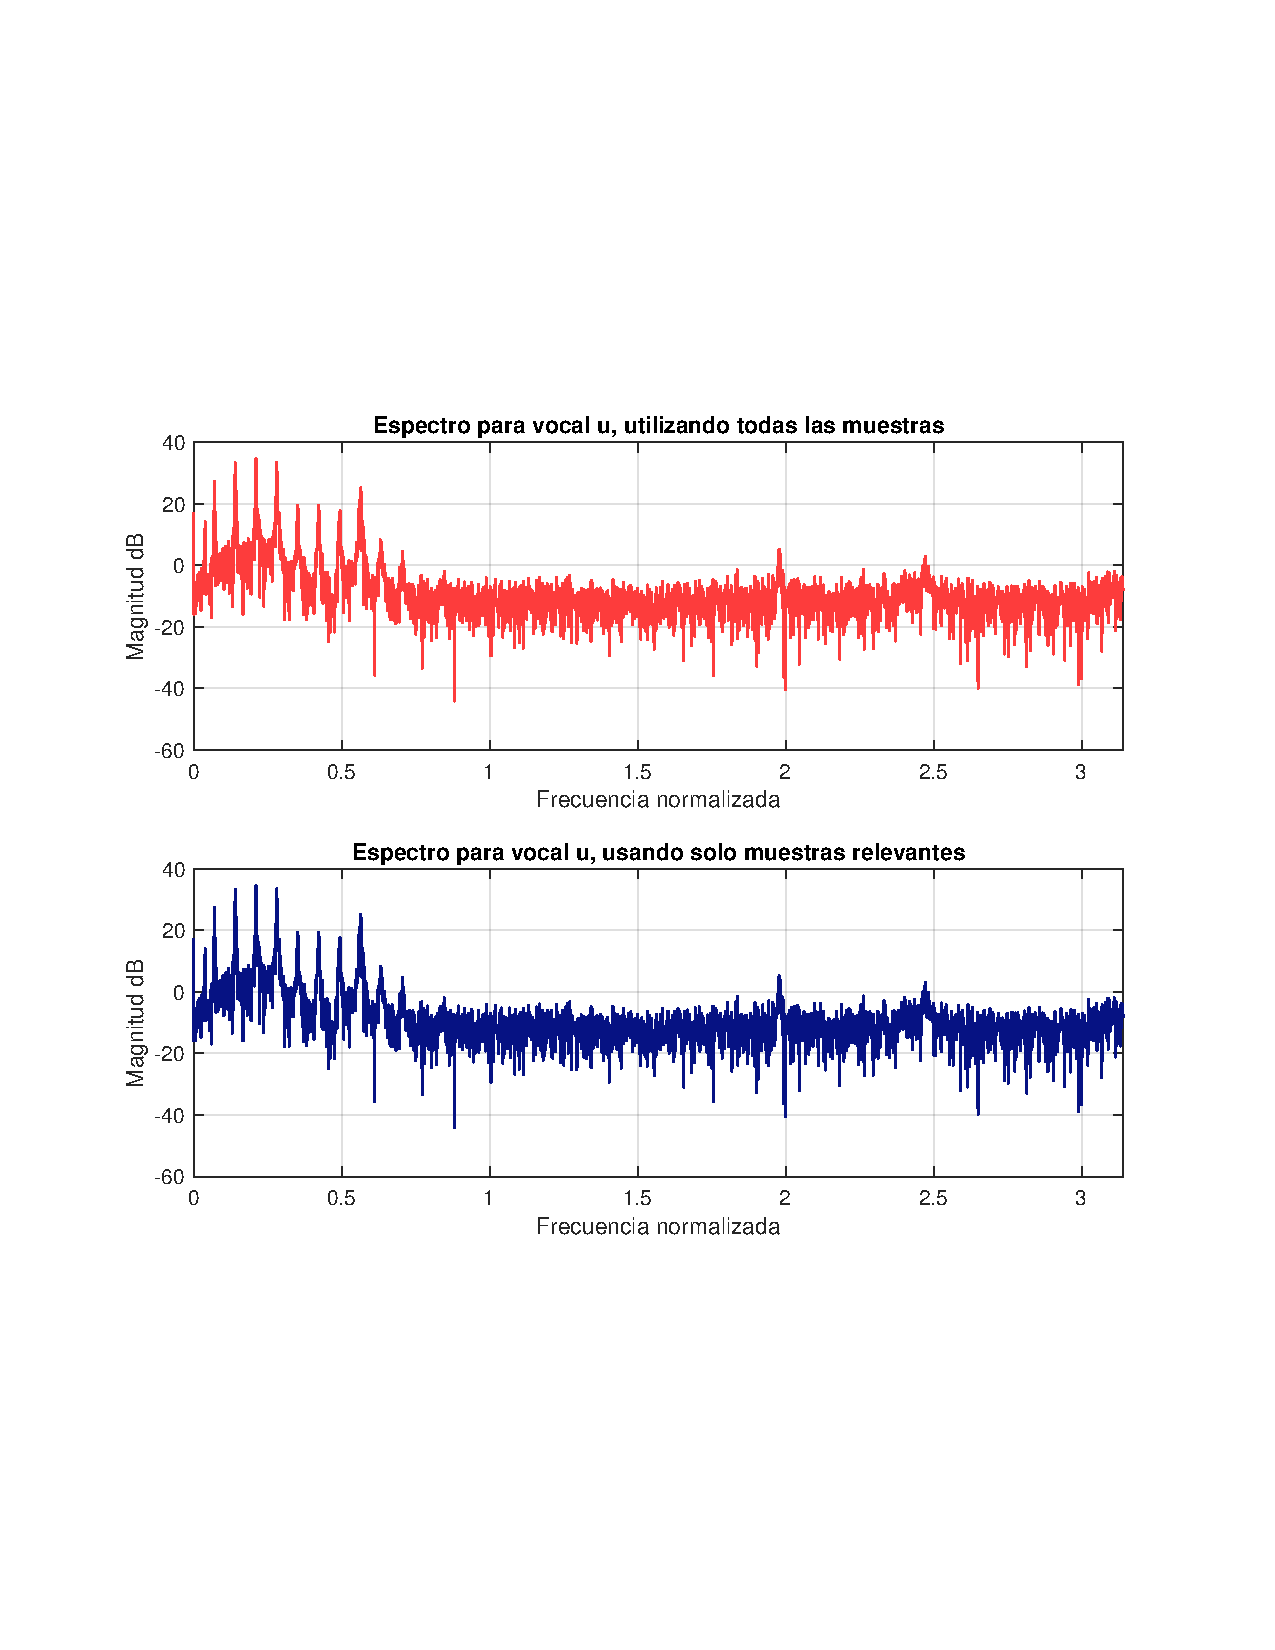
\includegraphics[width=0.6\textwidth,clip, trim = {1.9cm 6.8cm 2.3cm 7cm}]{../plots/u_fft.pdf}
		\caption{FFT para vocal u}
		\label{fig:u_fft}
	\end{figure}
	
	
	Analizando los resultados, se puede ver que, de manera visual, los espectros donde se consideró únicamente la porción que contenía información de la señal, se ve menos saturado, que para los que se consideró la señal completa. Esto se puede explicar, principalmente debido a que para las secciones donde la información de la vocal no se encuentra presente, no se tiene una situación de tipo \textit{zero-padding}, sino que se tiene ruido asociado al equipo de grabación. Por lo que al seleccionar únicamente la información de la señal, estamos limitando el ruido que se introduce al espectro. Es por esto, que se recomienda trabajar con la porción con información, dejando fuera los instantes donde solo hay \textit{ruido de background}.
	
	\subsection{Análisis de formantes}
	
	A partir de los gráficos obtenidos en el punto anterior, se procede a obtener la frecuencia fundamental de las vocales, además de sus primeras dos formantes, los resultados se entregan en la siguiente tabla:
	
	\begin{table}[H]
		\center
		\begin{tabular}{|c|c|c|c|}
			\hline
			\textbf{Vocal} & \textbf{Fundamental Hz} & \textbf{F1 Hz} & \textbf{F2 Hz} \\
			\hline 
			A & 87 & 796 & 1239 \\
			\hline
			E & 87 & 444 & 2037 \\
			\hline
			I & 87 & 175 & 2468 \\
			\hline
			O & 89 & 444 & 886 \\
			\hline
			U & 89 & 267 & 719 \\
			\hline
		\end{tabular}
		\caption{Tabla de frecuencia fundamental y formantes, para las distintas vocales}
		\label{tab:formantes-freq}
	\end{table}
	
	Graficando F1 v/s F2, para generar el triángulo vocálico:

	\begin{figure}[H]
		\center
		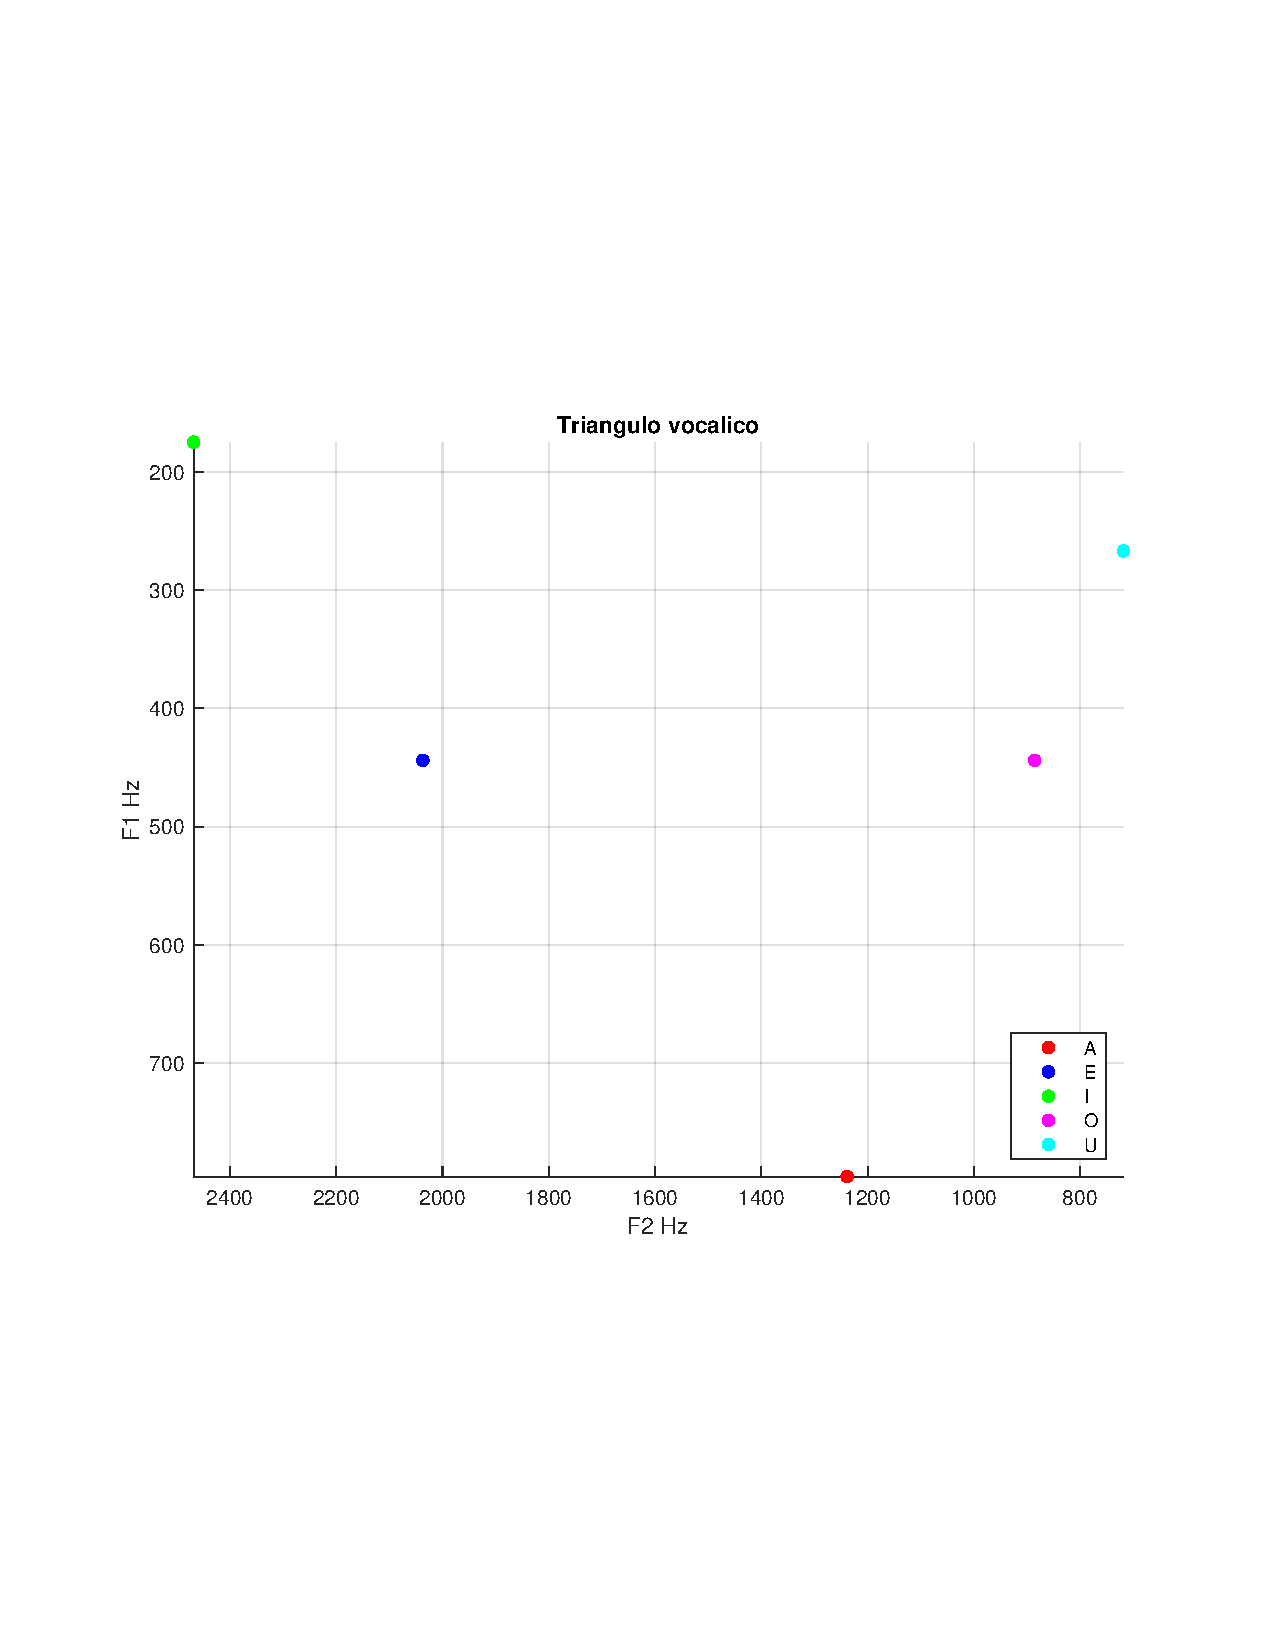
\includegraphics[width=0.6\textwidth,clip, trim = {1.9cm 6.8cm 2.3cm 7cm}]{../plots/vocalic_triang.pdf}
		\caption{Triángulo vocálico obtenido}
		\label{fig:vocal_triang}
	\end{figure}
	
	Note que para generarlo, se tiene que invertir la dirección de los ejes, dado que se define el origen en la esquina superior derecha. Comparando este resultado con el esperado de forma teórica, se puede ver que se comporta de manera similar:
	\begin{figure}[H]
		\center
		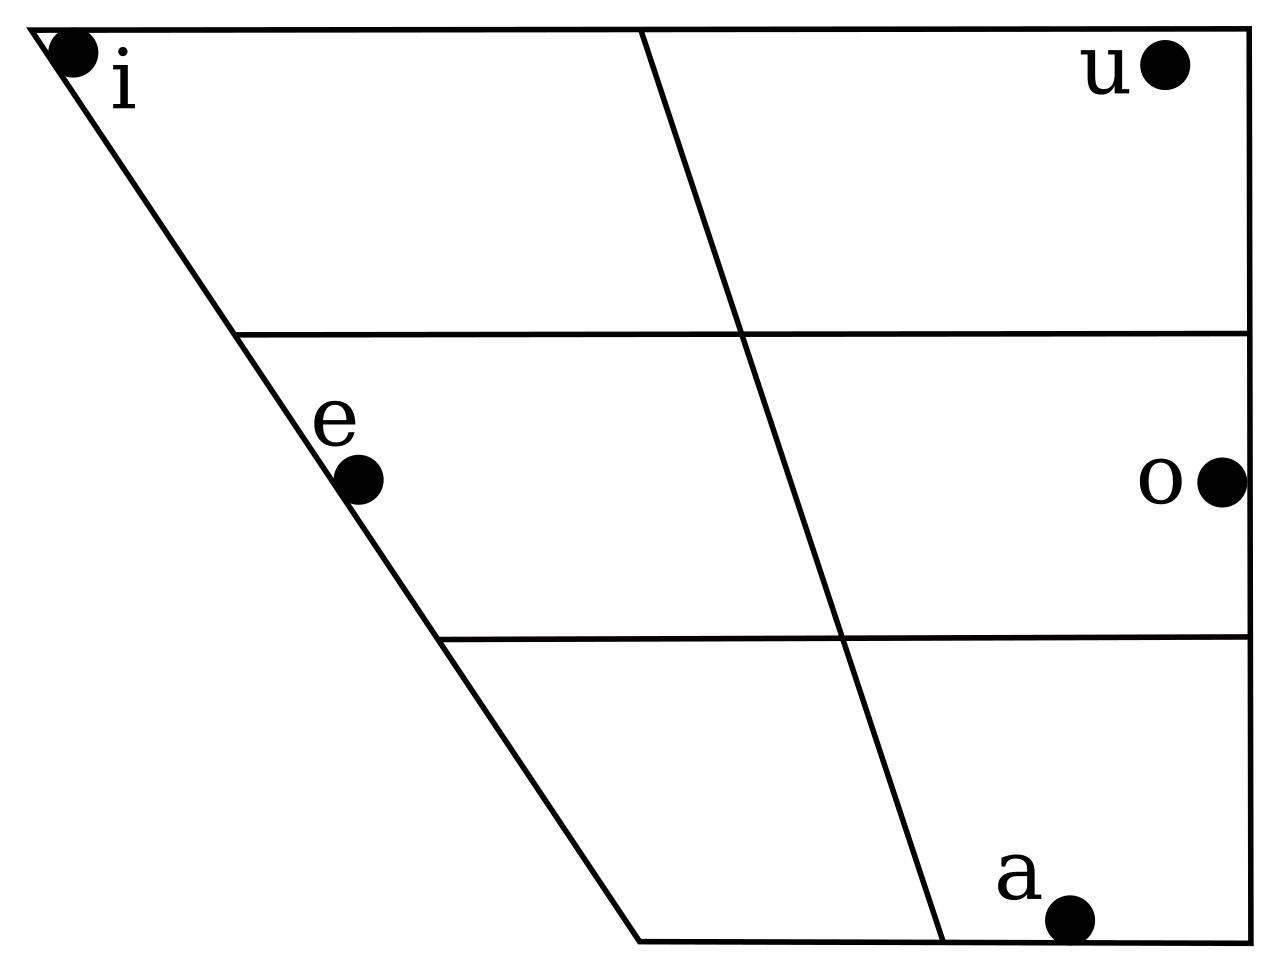
\includegraphics[width = 0.6\linewidth]{../plots/1280px-Spanish_vowel_chart.png}
		\caption{Triángulo vocálico teórico. Cortesía de Wikipedia}
		\label{fig:triang_vocal_teorico}
	\end{figure}
	
	
	\subsection{LPC}
		Utilizando la función \texttt{lpc(x,p)} de \textsc{Matlab} se procede a obtener los filtros IIR asociados a cada vocal. Graficando la magnitud de su respuesta en frecuencia y comparando con el espectro de la vocal se obtiene:
		
	
	\begin{figure}[H]
		\center
		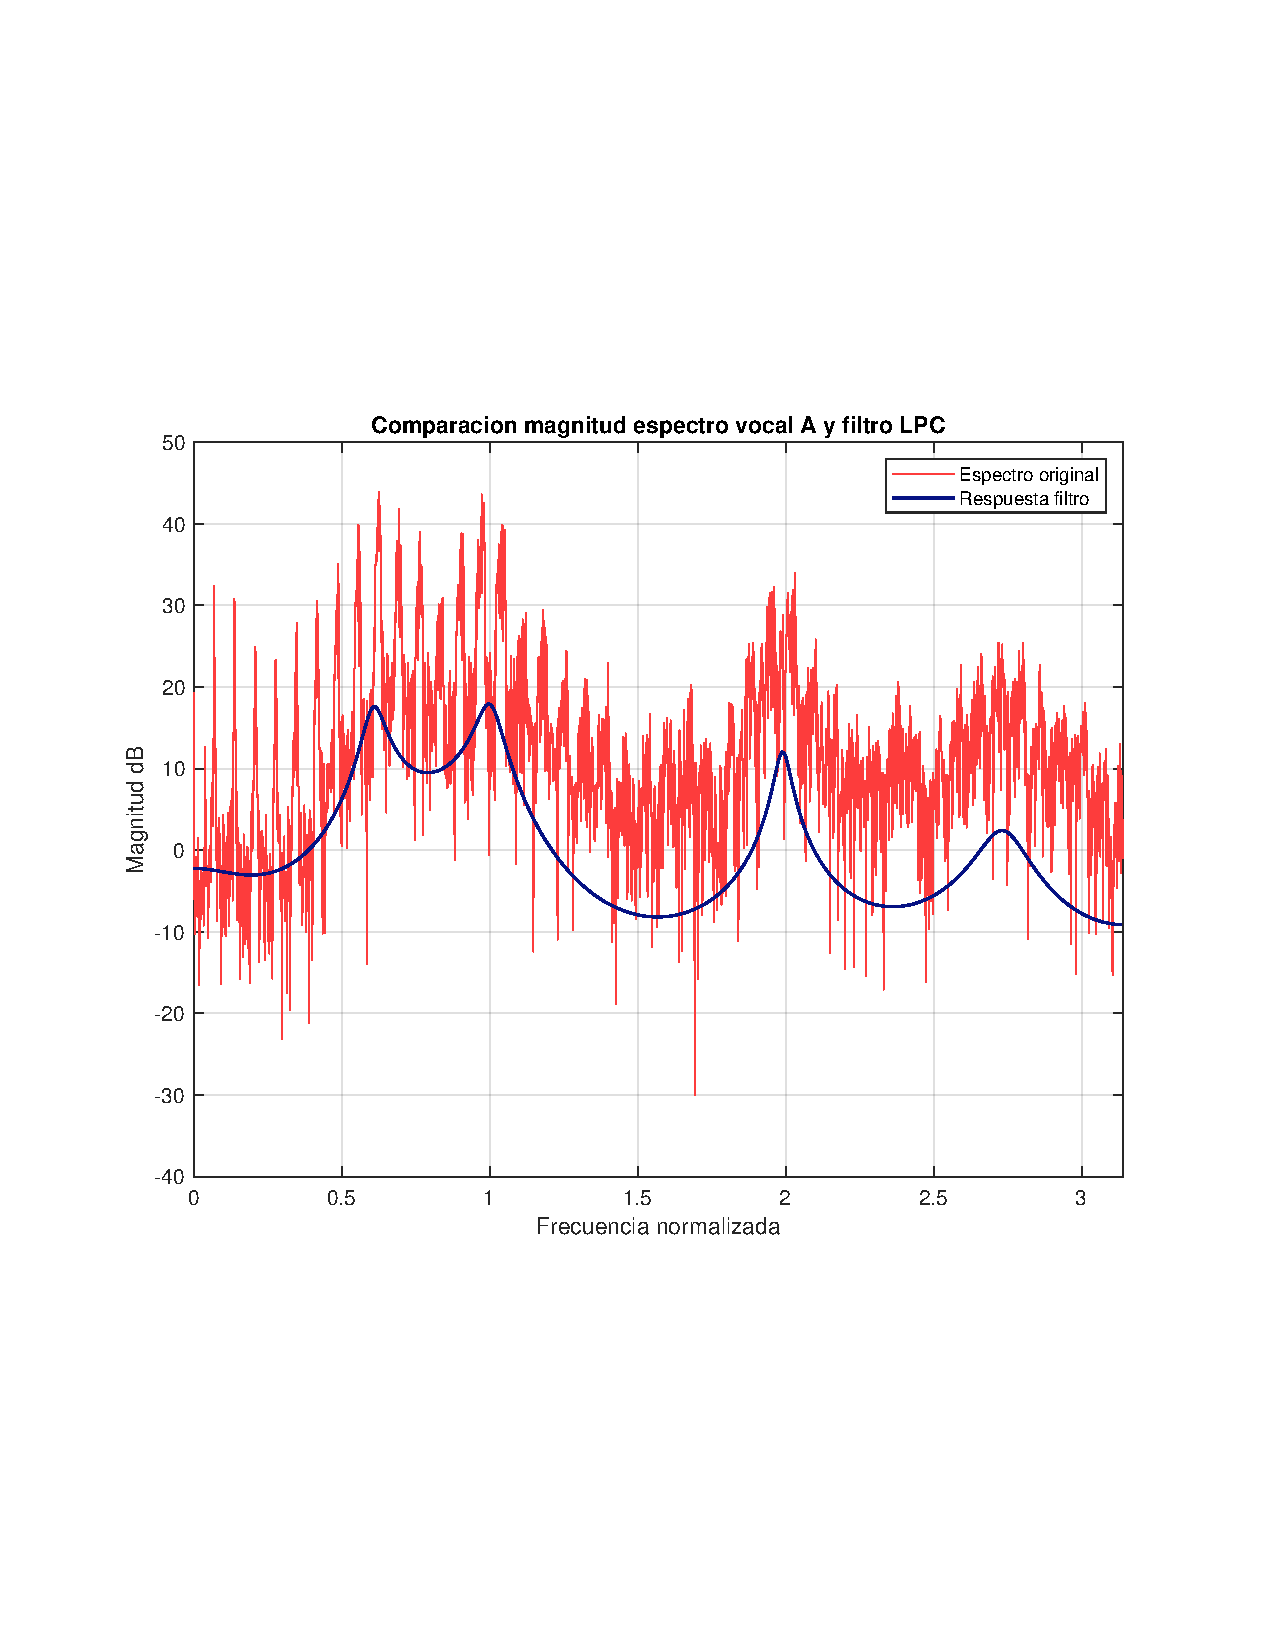
\includegraphics[width=0.6\textwidth,clip, trim = {1.9cm 6.8cm 2.3cm 7cm}]{../plots/A_lpc.pdf}
		\caption{Comparación espectro y filtro LPC: A}
		\label{fig:LPC_A}
	\end{figure}

	\begin{figure}[H]
		\center
		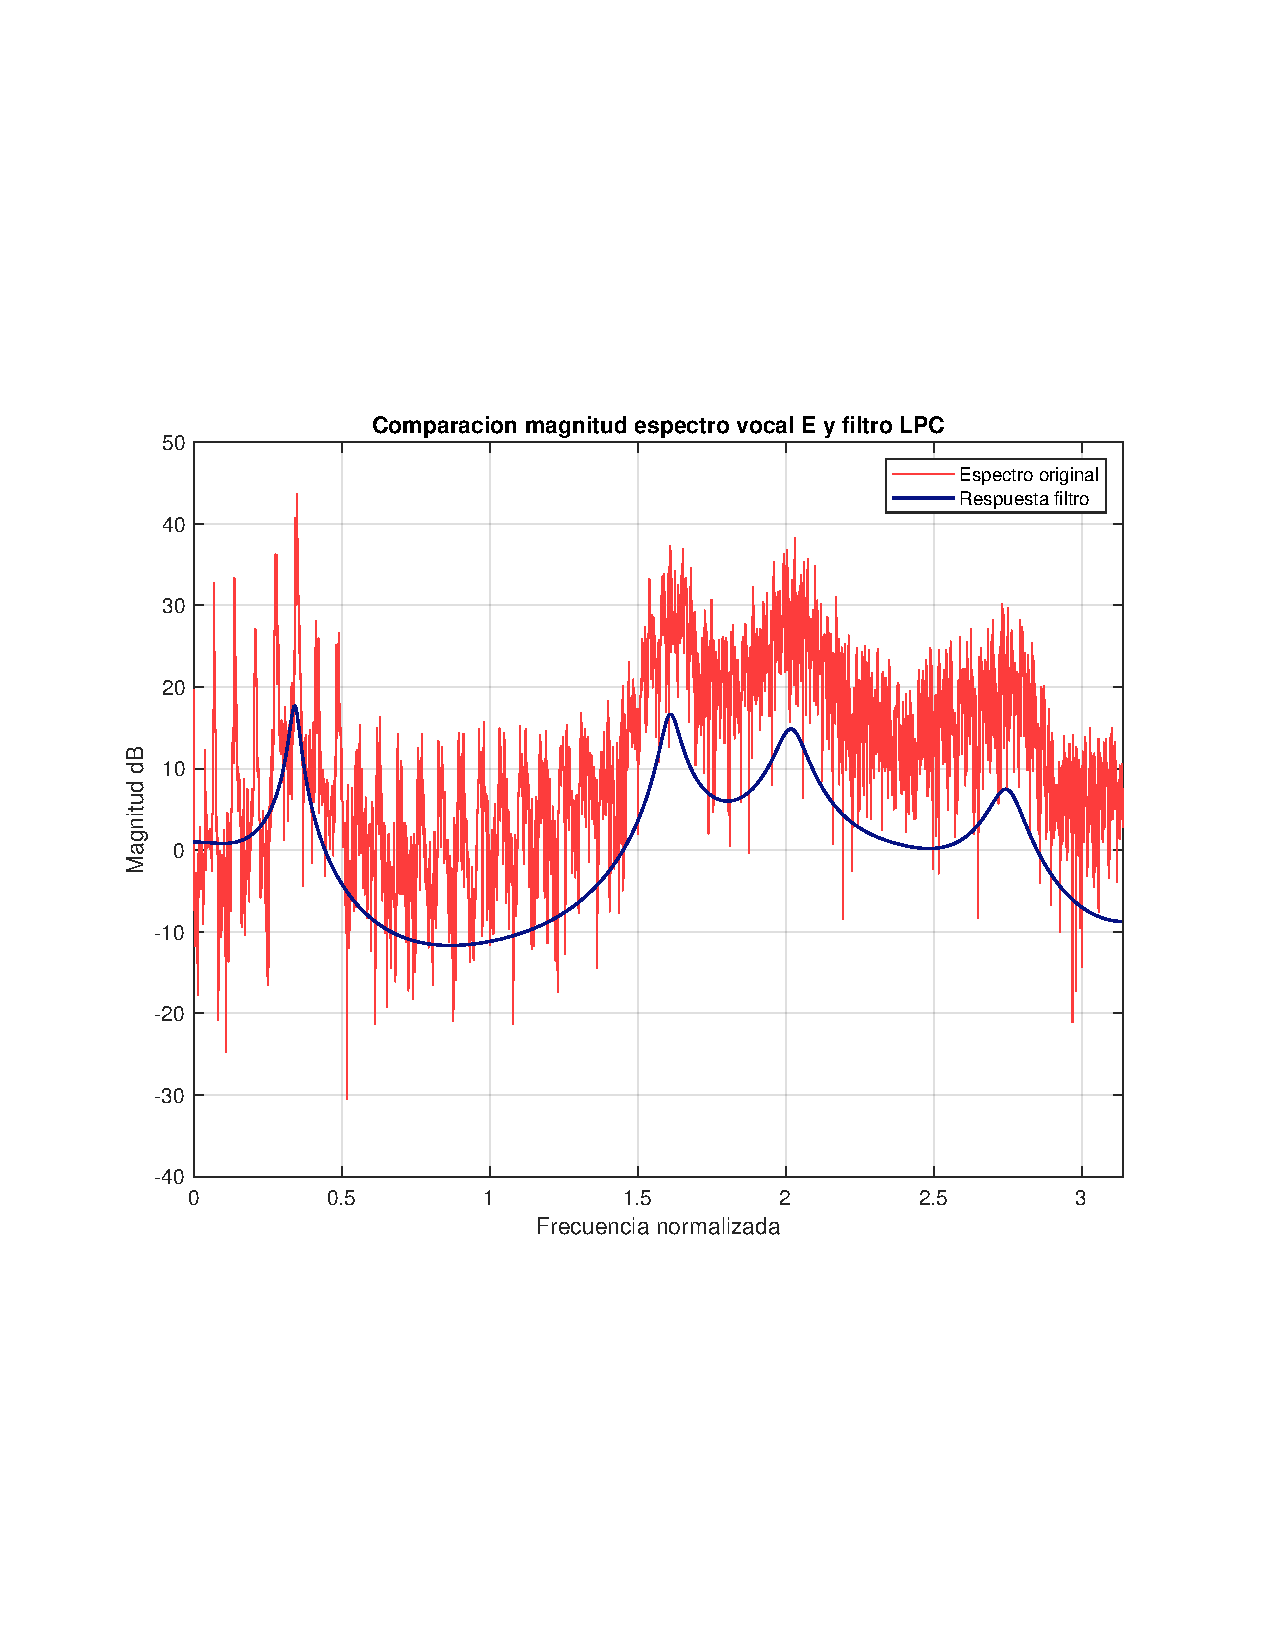
\includegraphics[width=0.6\textwidth,clip, trim = {1.9cm 6.8cm 2.3cm 7cm}]{../plots/E_lpc.pdf}
		\caption{Comparación espectro y filtro LPC: E}
		\label{fig:LPC_E}
	\end{figure}

	\begin{figure}[H]
		\center
		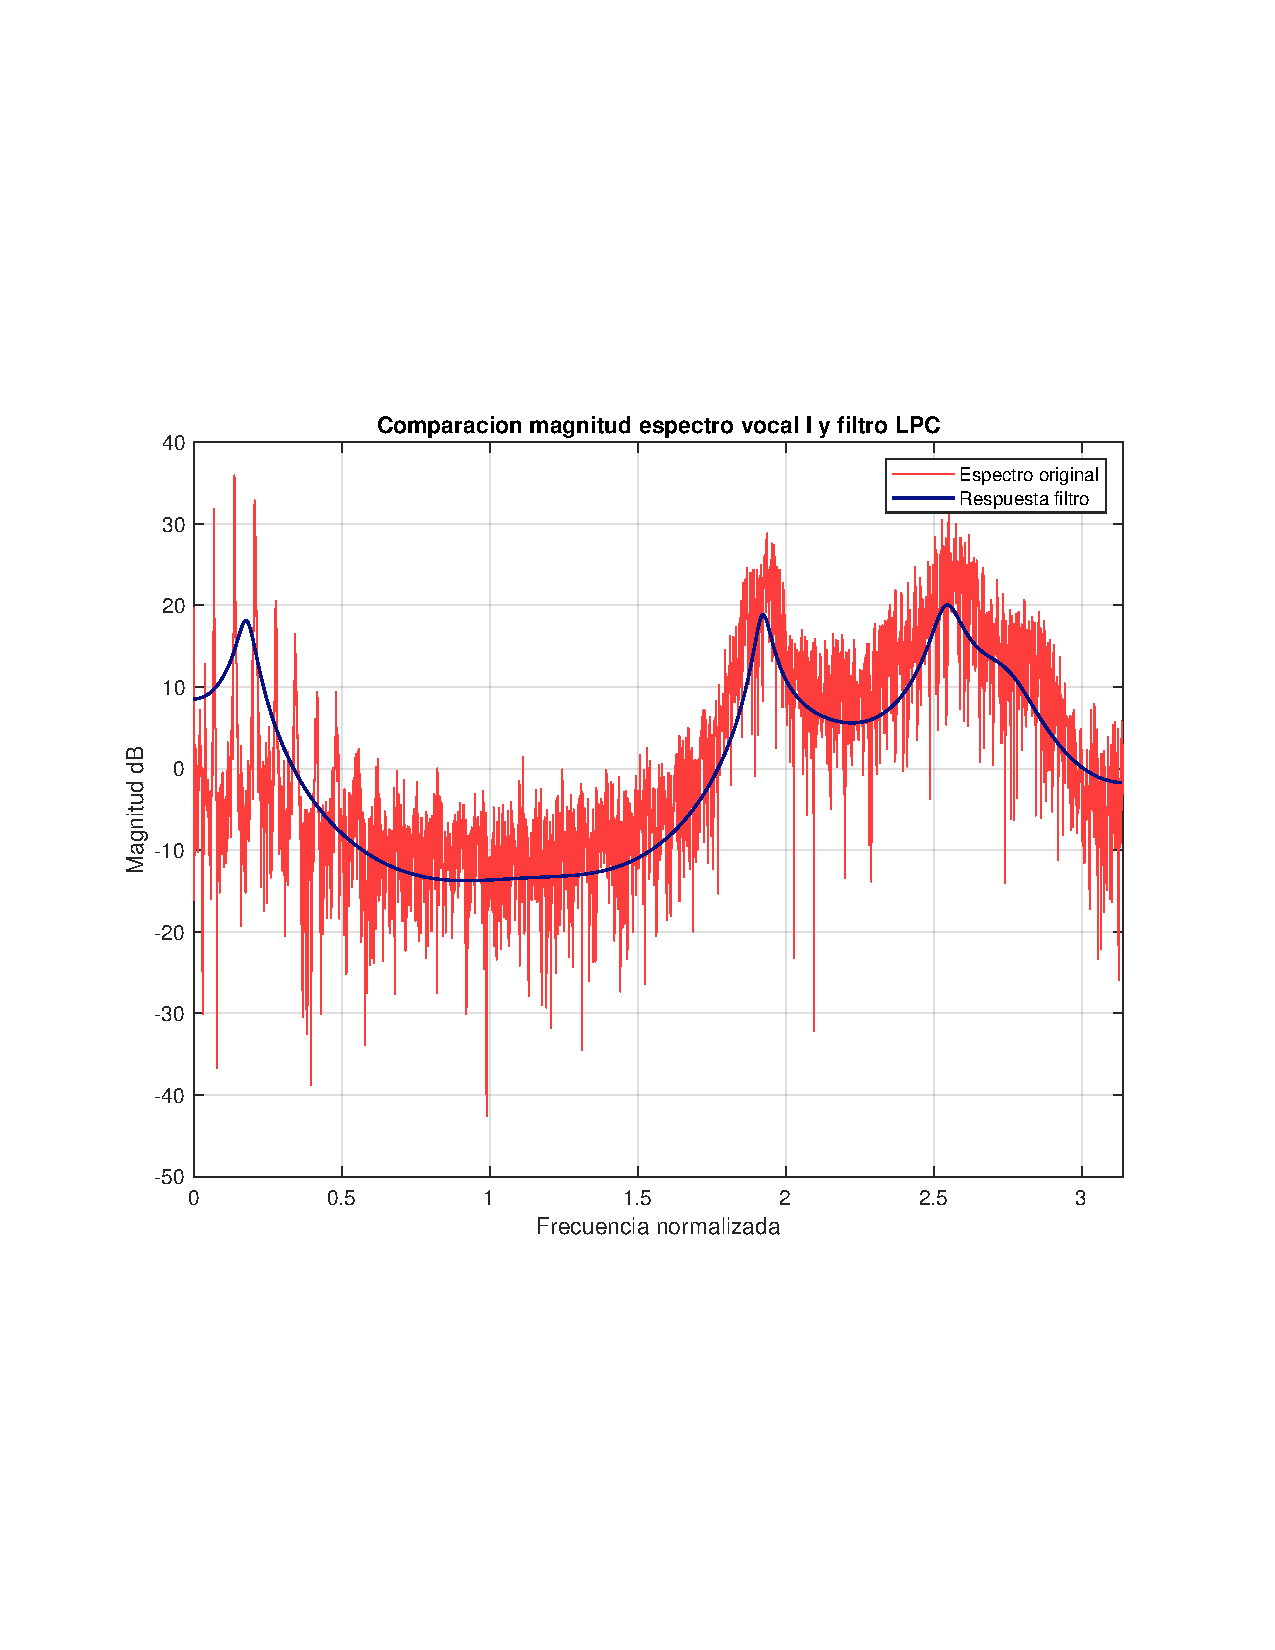
\includegraphics[width=0.6\textwidth,clip, trim = {1.9cm 6.8cm 2.3cm 7cm}]{../plots/I_lpc.pdf}
		\caption{Comparación espectro y filtro LPC: I}
		\label{fig:LPC_I}
	\end{figure}

	\begin{figure}[H]
		\center
		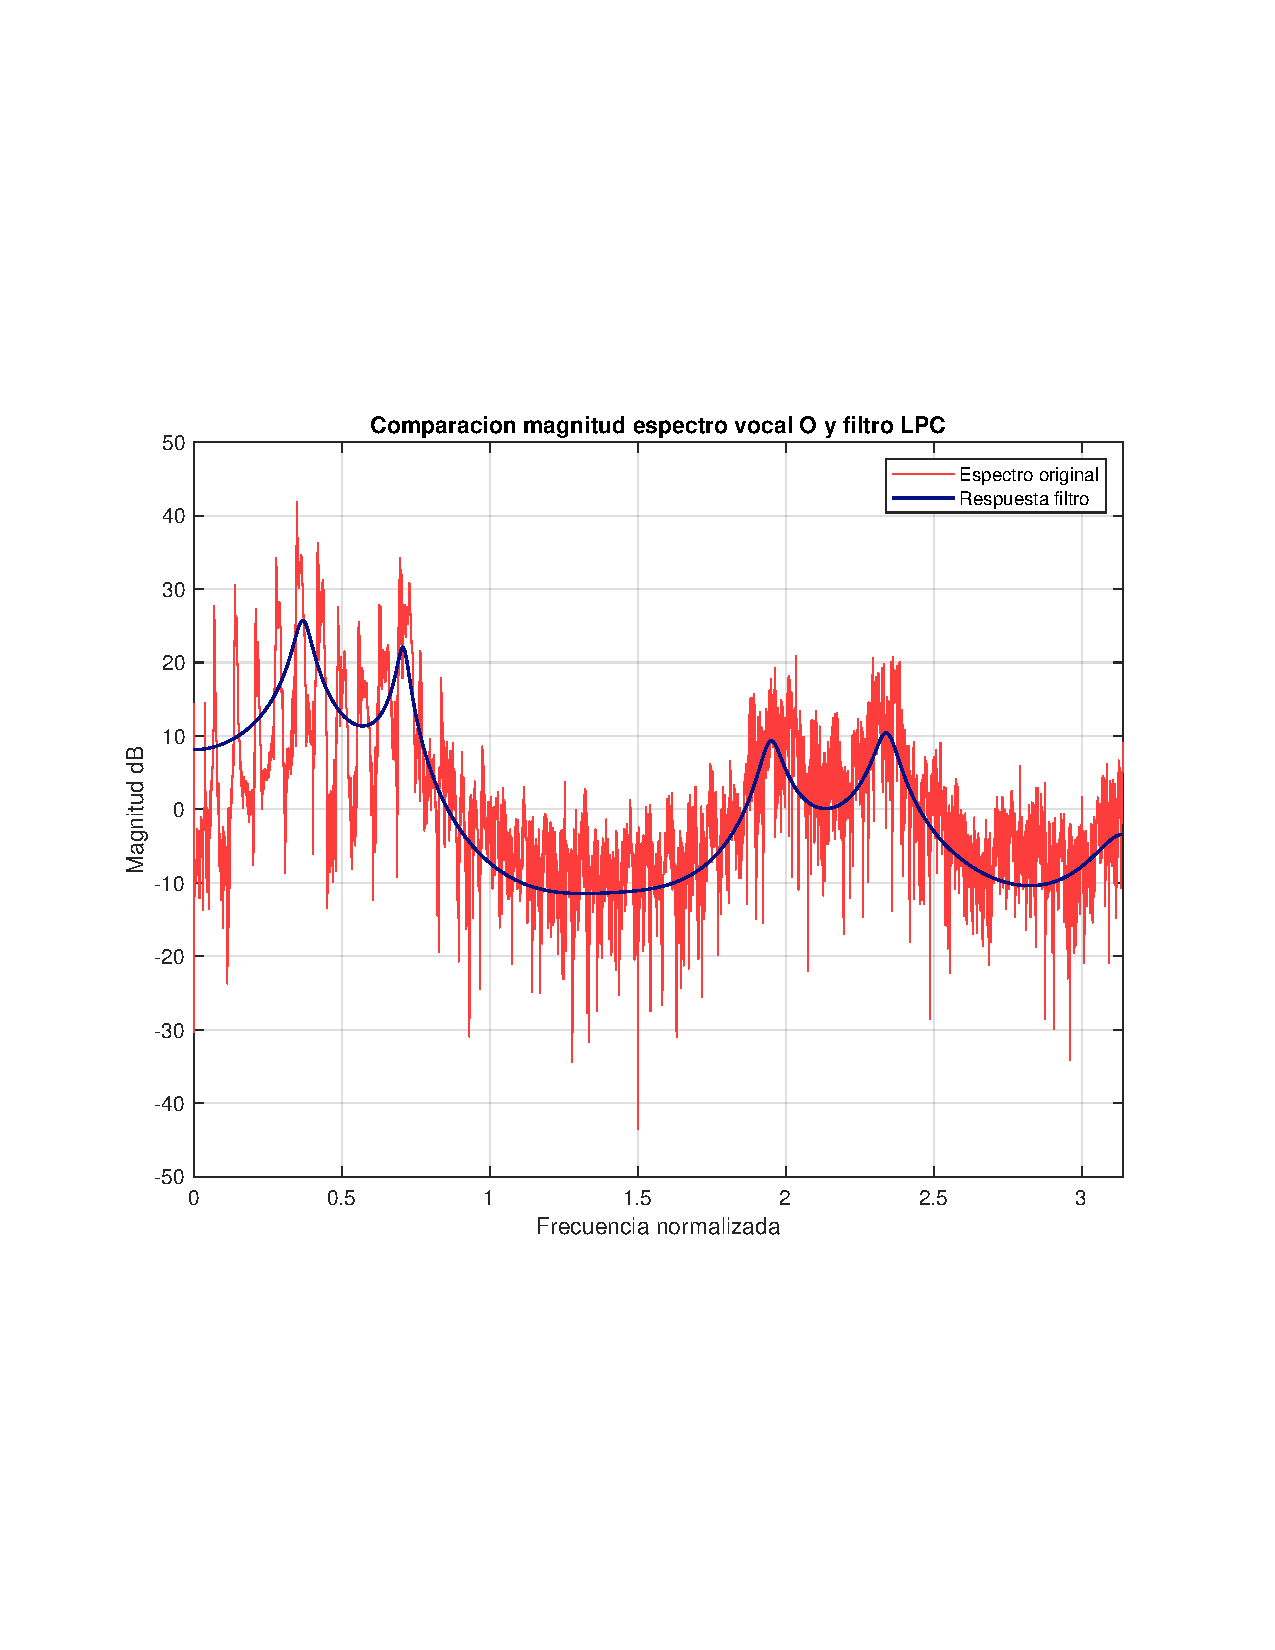
\includegraphics[width=0.6\textwidth,clip, trim = {1.9cm 6.8cm 2.3cm 7cm}]{../plots/O_lpc.pdf}
		\caption{Comparación espectro y filtro LPC: O}
		\label{fig:LPC_O}
	\end{figure}

	\begin{figure}[H]
		\center
		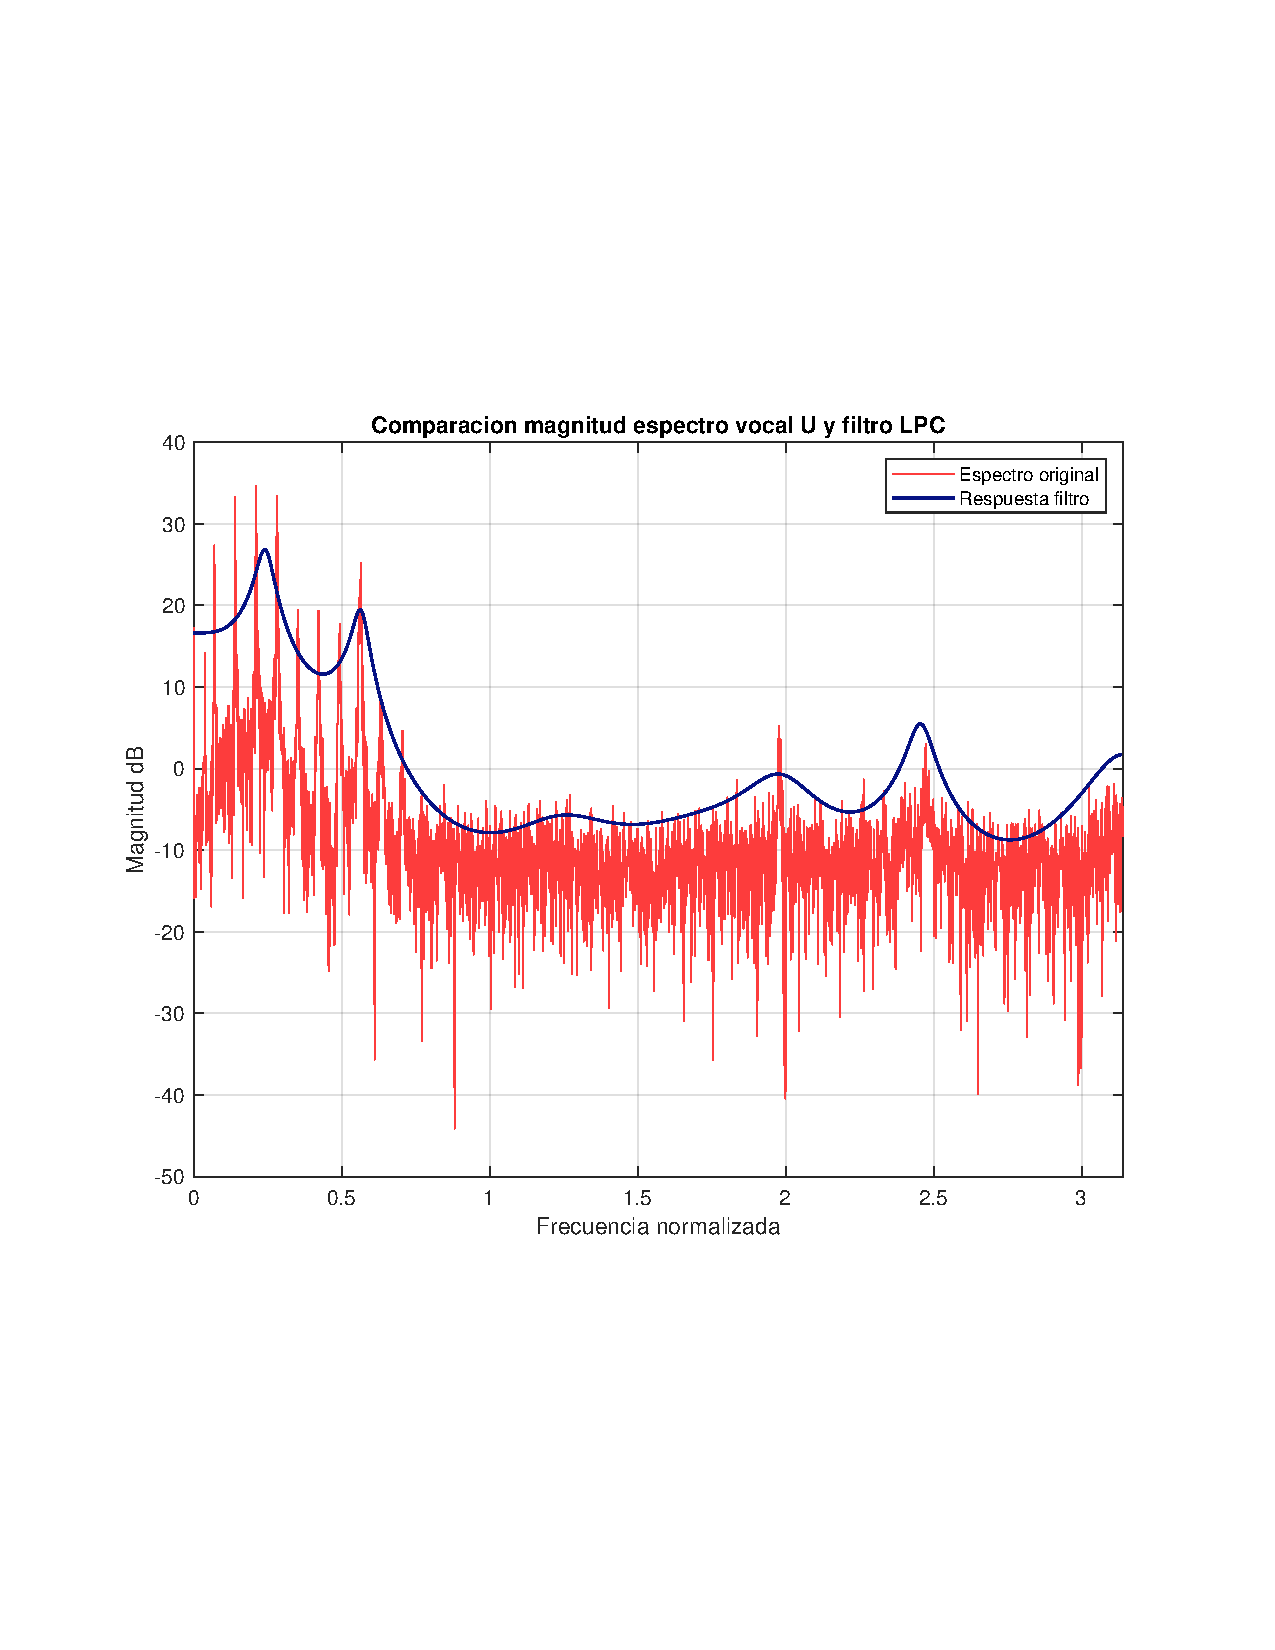
\includegraphics[width=0.6\textwidth,clip, trim = {1.9cm 6.8cm 2.3cm 7cm}]{../plots/U_lpc.pdf}
		\caption{Comparación espectro y filtro LPC: U}
		\label{fig:LPC_U}
	\end{figure}
	
	Se puede ver, que el resultado del filtro obtenido mediante LPC, permite tener una respuesta similar a la envolvente de la magnitud del espectro de la vocal. A partir de esto, se vuelve a obtener las formantes para cada vocal:
	\begin{table}[H]
		\center
		\begin{tabular}{|c|c|c|}
			\hline
			\textbf{Vocal}  & \textbf{F1 Hz} & \textbf{F2 Hz} \\
			\hline 
			A & 772 & 1273 \\
			\hline
			E & 420 & 2050 \\
			\hline
			I & 225 & 2444 \\
			\hline
			O & 468 & 898 \\
			\hline
			U & 304 & 718\\
			\hline
		\end{tabular}
		\caption{Tabla de frecuencia fundamental y formantes, para las distintas vocales, obtenidas mediante LPC}
		\label{tab:formantes-freq_lpc}
	\end{table}
	
	Comparando con lo obtenido en el punto anterior, tabla \ref{tab:formantes-freq}, se puede ver que los valores se mantuvieron aproximadamente constantes, graficando un nuevo triangulo vocálico:
	\begin{figure}[H]
		\center
		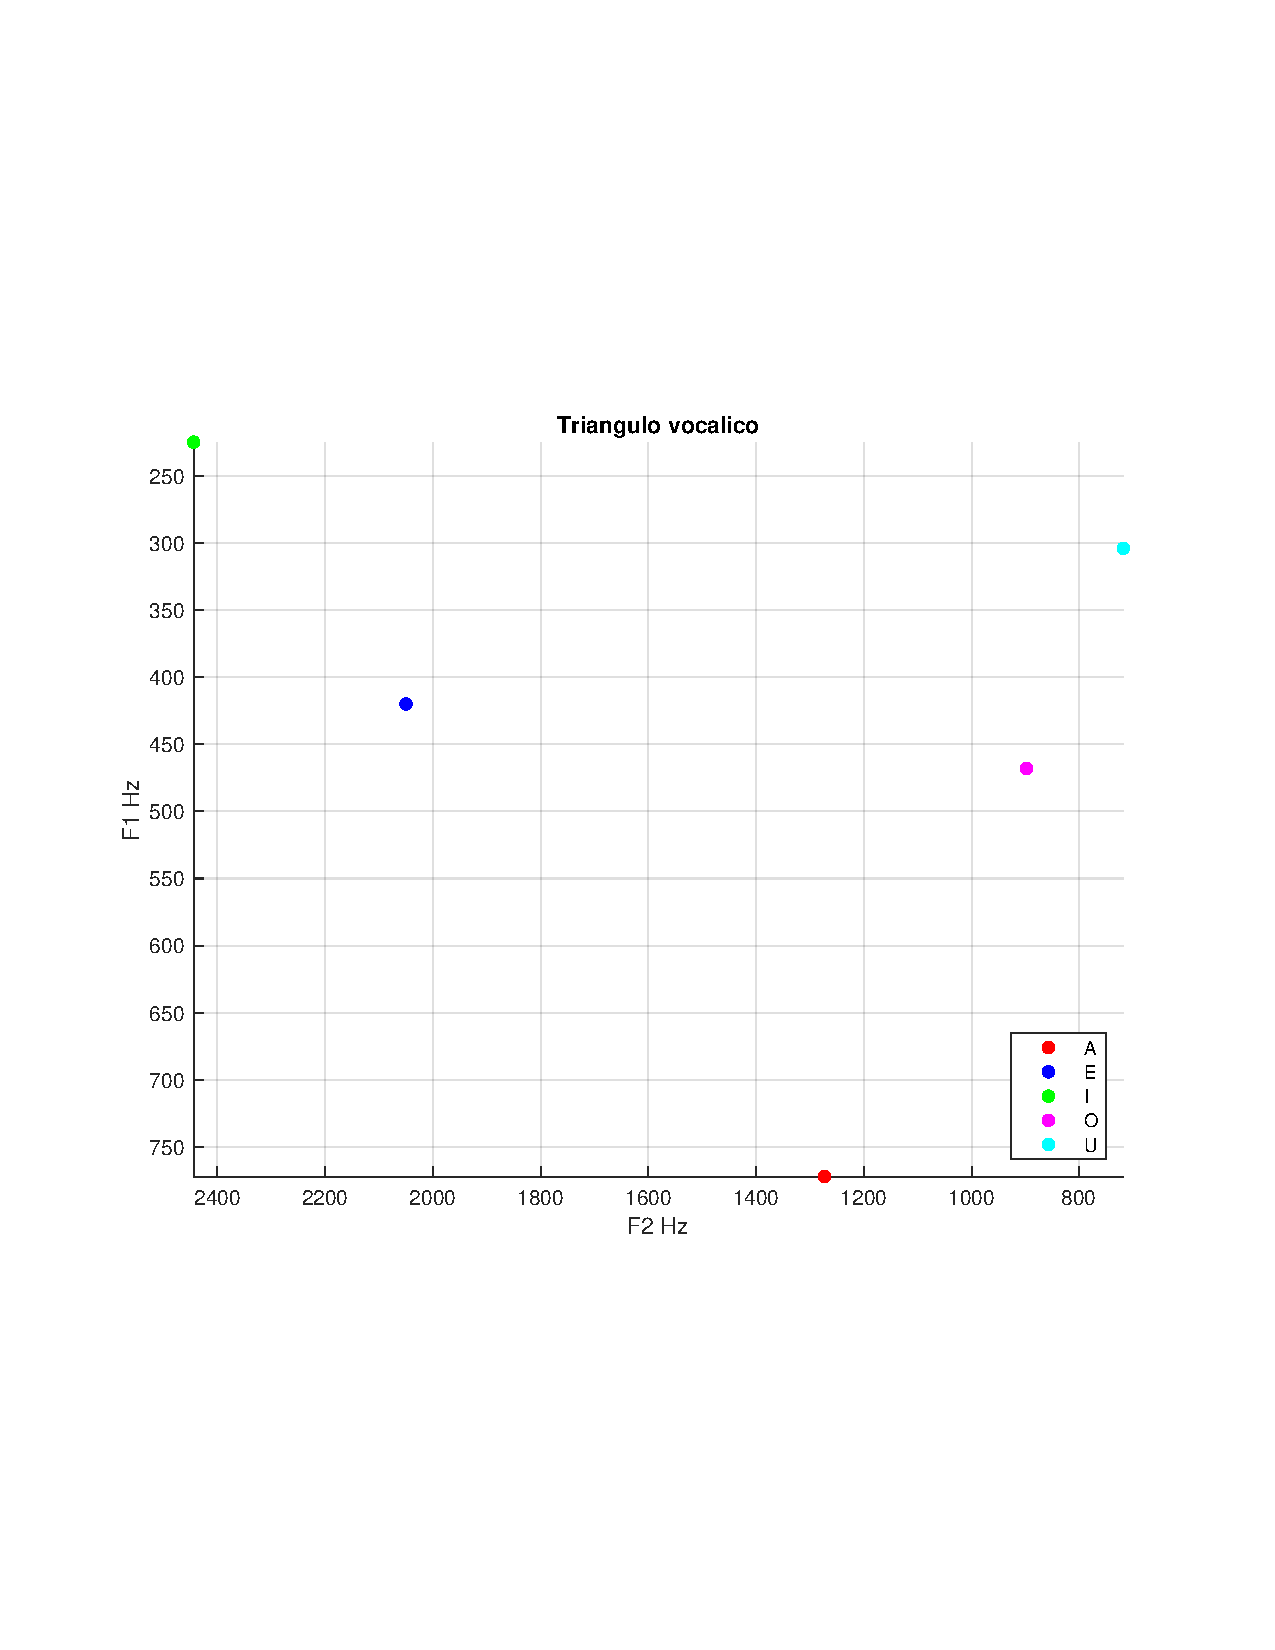
\includegraphics[width=0.6\textwidth,clip, trim = {1.9cm 6.8cm 2.3cm 7cm}]{../plots/vocalic_triang_2.pdf}
		\caption{Triángulo vocálico obtenido mediante LPC}
		\label{fig:vocal_triang_LPC}
	\end{figure}
	
	Realizando la comparación directa con el triangulo obtenido en figura \ref{fig:vocal_triang}:
	\begin{figure}[H]
		\center
		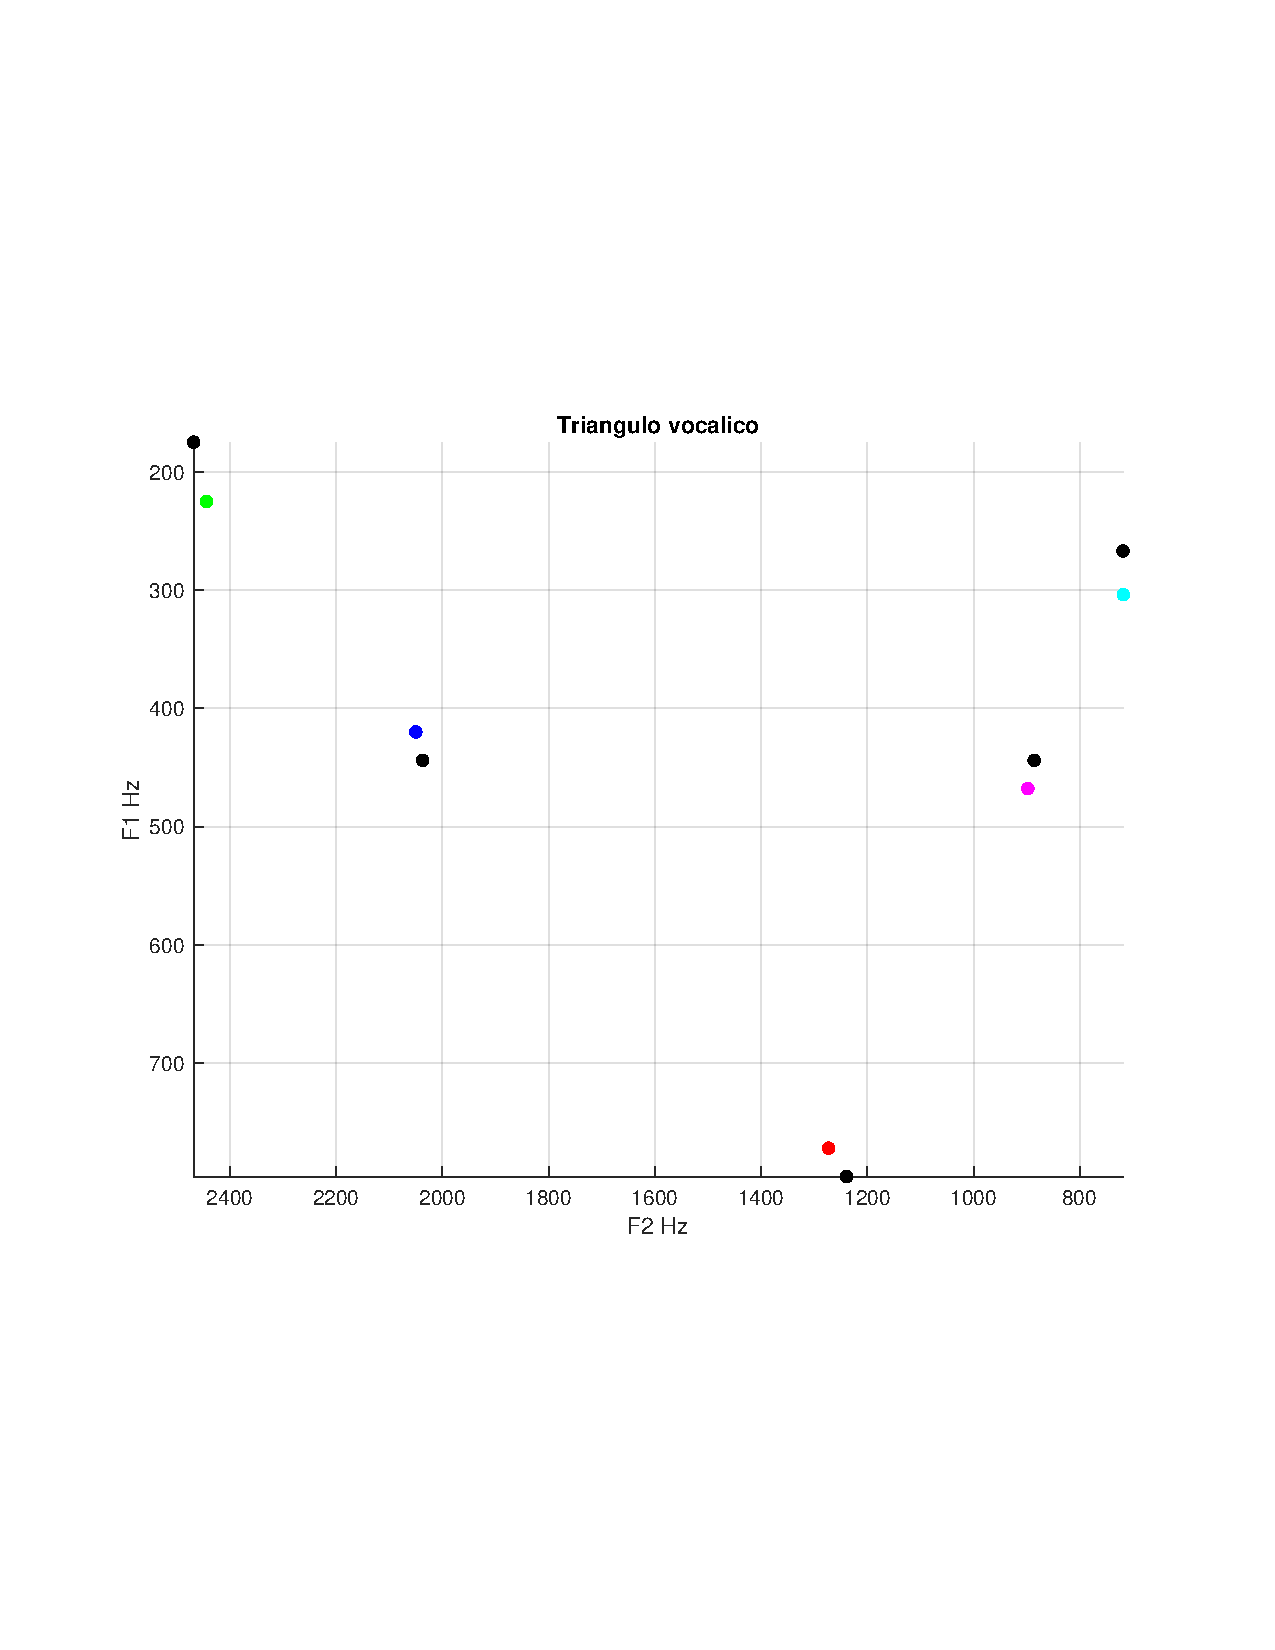
\includegraphics[width=0.6\textwidth,clip, trim = {1.9cm 6.8cm 2.3cm 7cm}]{../plots/vocalico_comp.pdf}
		\caption{Comparación triángulo vocálico obtenido mediante LPC (en colores) y comparación triangulo obtenido desde el espectro (negro).}
		\label{fig:vocal_triang_LPC_comparative}
	\end{figure}
	
	A partir de esto, se puede ver que el movimiento de las formantes, para las vocales es mínimo y siguen estando bastante cerca de las formantes obtenidas del espectro, por lo que se puede concluir que el filtro representa de manera fiel la envolvente asociada al espectro de cada vocal.
	